% id: 19-14
% book: 베이직쎈 확률과 통계 · 01 여러 가지 순열
% section: 실전 감각 UP
% figure: tikz:fig-19-14
% answer: 
% answer_source: 
% variant_level: 0 (원본 전사)
% 이 파일은 build.mjs 가 items.json 에서 만든다. 고칠 때는 items.json 을 고친다.
\smash{\raisebox{1.5mm}{\dmkichul{베이직쎈 확률과 통계 19쪽 14번}}}
다음 그림과 같이 도로망이 $\pt{P}$에서 서로 연결되어 있다. $\pt{A}$에서 $\pt{B}$까지 최단 거리로 가는 경우의 수를 구하시오.
\par\smallskip\begin{center}\resizebox{\ifdim\width>\linewidth\linewidth\else\width\fi}{!}{% 19-14(19쪽) — P 에서 서로 연결된 두 도로망(45도로 놓인 격자 · 왼쪽 2×3칸 · 오른쪽 2×2칸)과 지점 A, P, B.
% 스캔 화질이 낮아 TikZ 로 다시 그림(라벨은 원문에 있는 A, P, B 뿐 · 경우의 수는 그림에 적지 않는다).
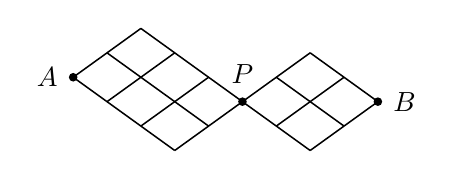
\begin{tikzpicture}[x={(0.43cm,0.31cm)},y={(0.43cm,-0.31cm)},line width=0.55pt]
  % 왼쪽 도로망: A(0,0) 에서 북동 2칸 · 남동 3칸
  \foreach \i in {0,1,2} \draw (\i,0) -- (\i,3);
  \foreach \j in {0,1,2,3} \draw (0,\j) -- (2,\j);
  % 오른쪽 도로망: P(2,3) 에서 북동 2칸 · 남동 2칸
  \foreach \i in {2,3,4} \draw (\i,3) -- (\i,5);
  \foreach \j in {3,4,5} \draw (2,\j) -- (4,\j);
  \node[fill,circle,inner sep=1.1pt] at (0,0) {};
  \node[fill,circle,inner sep=1.1pt] at (2,3) {};
  \node[fill,circle,inner sep=1.1pt] at (4,5) {};
  \node[left=2pt] at (0,0) {$\pt{A}$};
  \node[above=3pt] at (2,3) {$\pt{P}$};
  \node[right=2pt] at (4,5) {$\pt{B}$};
\end{tikzpicture}
}\end{center}
